\documentclass{article}
\usepackage[margin=.9in]{geometry}
\usepackage[dvipsnames]{xcolor}
\usepackage{amsmath}
\usepackage{amssymb}
\usepackage{amsthm}
\usepackage{tikz}
\usepackage{mathrsfs}
\usepackage{float}
\newtheorem*{claim}{Claim}
\newtheorem*{poof}{Proof}
\title{HW 7}
\author{Christopher Hunt}
\date{}
\usepackage{graphicx} 
\usepackage{fancyhdr}

\begin{document}
\pagestyle{fancy}
\fancyhf{}
\rfoot{MTH 231}
\lfoot{Christopher Hunt}
\lhead{HW 7}
\rhead{\thepage}
\maketitle

\section*{15. Prove that any graph with at least two vertices must have two vertices of the same degree.}
\begin{claim}
    Any graph with at least two vertices must have two vertices of the same degree.
\end{claim}
\begin{poof}
    Concider a graph $G$ where this is not the case. $G$ is a graph that contains $n > 1$ vertices where every vertex has a unique number of degrees. The set of degrees of each vertex would be:
    \[\{0,1,2,3,...,n-2,n-1\}\]
    The range of degree values is from $0$ to $n-1$. No vertex can have less than zero degrees and no vertex can have more degrees than there are other vertices besides the vertex being examined. This means that there are $n$ amount of possible unique degree values, therefore each vertex must have a degree from within this range. Examining this scenario we find that this graph must contain a vertex that is not connected to any other vertex (degree $0$) while also having a vertex connected to every other vertex in the graph (degree $n-1$), which includes the vertex of degree 0. This is a contradiction. Therefore, by contradiction, the claim is proved to be true.\\
    \qed\end{poof}

\newpage
\section*{7.The two problems below can be solved using graph coloring. For each problem, represent the situation with a graph, say whether you should be coloring vertices or edges and why, and use the coloring to solve the problem.}
For this problem I will color the edges. Each color of edge represents a day a match is played.

\subsection*{a. Your Quidditch league has 5 teams. You will play a tournament next week in which every team will play every other team once. Each team can play at most one match each day, but there is plenty of time in the day for multiple matches. What is the fewest number of days over which the tournament can take place?}
To solve this we will use colored edges to represent the days where the two adjacent teams played. Since there are only five teams and teams can only play one match per day there can only ever be two matchs played by 4 different teams each day, since the 5th would have to play a team that already played that day. Start by drawing edges between teams who have played. Day 1 is red, teams 1 and 2 play and 3 and 5 play. Day 2 is green, team 1 and team 3 play and team 2 and team 4 play. Day 3 is orange, team 2 plays team 3 and team 4 plays team 5. Day 4 is yellow, team 2 plays team 5 and team 1 plays team 4. Day 5 is blue, team 1 plays team 5 and team 3 plays team 4. At this point every team has played every other team, it took 5 days. 
\begin{center}
    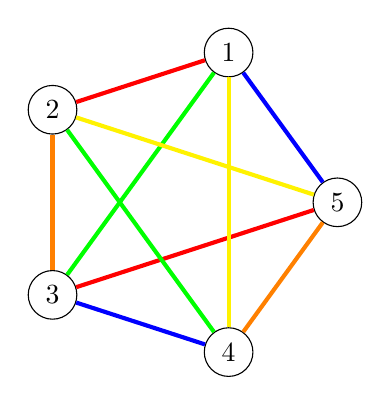
\begin{tikzpicture}
        \foreach \i in {1,...,5} {
          \node[circle, draw] (\i) at (72*\i:2) {\i};
        }
        \draw[line width=1.5pt, color=red] (2) -- (1);
        \draw[line width=1.5pt, color=red] (3) -- (5);
        \draw[line width=1.5pt, color=green] (1) -- (3);
        \draw[line width=1.5pt, color=green] (2) -- (4);
        \draw[line width=1.5pt, color=orange] (2) -- (3);
        \draw[line width=1.5pt, color=orange] (4) -- (5);
        \draw[line width=1.5pt, color=yellow] (2) -- (5);
        \draw[line width=1.5pt, color=yellow] (1) -- (4);
        \draw[line width=1.5pt, color=blue] (1) -- (5);
        \draw[line width=1.5pt, color=blue] (3) -- (4);
    \end{tikzpicture}
\end{center}

\subsection*{b. Ten members of Math Club are driving to a math conference in a neighboring state. However, some of these students have dated in the past, and things are still a little awkward. Each student lists which other students they refuse to share a car with; these conflicts are recorded in the table below. What is the fewest number of cars the club needs to make the trip? Do not worry about running out of seats, just avoid the conflicts.}

\begin{center}
    \begin{tabular}{|c|c|c|c|c|c|c|c|c|c|c|}
        \hline
        \textbf{Student} & A & B & C & D & E & F & G & H & I & J \\
        \hline
        \textbf{Conflicts} & BEJ & ADG & HJ & BF & AI & DJ & B & CI & EHJ &ACFI \\
        \hline
    \end{tabular}
    \end{center}
    
For this problem we will color the vertices. Each color represents which car the student will go in. The graph will be made of student vertices and conflicting adjacencies. The graph of the conflics creates a planar graph with three cycles, two even and one odd, with an additional vertex as a spike. The two even cycles could be handled with two cars but since there is an odd cycle we must add an additional car or else there would be a conflict between two vertices.
\begin{center}
    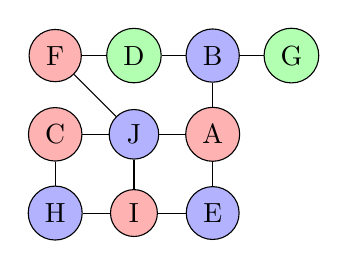
\begin{tikzpicture}
        % Draw vertices
        \node[circle, draw, fill=red!30] (00) at (0, 0) {F};
        \node[circle, draw, fill=green!30] (01) at (1, 0) {D};
        \node[circle, draw, fill=blue!30] (02) at (2, 0) {B};
        \node[circle, draw, fill=green!30] (03) at (3, 0) {G};
        \node[circle, draw, fill=red!30] (10) at (0, -1) {C};
        \node[circle, draw, fill=blue!30] (11) at (1, -1) {J};
        \node[circle, draw, fill=red!30] (12) at (2, -1) {A};
        \node[circle, draw, fill=blue!30] (20) at (0, -2) {H};
        \node[circle, draw, fill=red!30] (21) at (1, -2) {I};
        \node[circle, draw, fill=blue!30] (22) at (2, -2) {E};
      
        % Draw edges
        \draw (00) -- (01) -- (02) -- (03);
        \draw (00) -- (11);
        \draw (10) -- (11) -- (12);
        \draw (20) -- (21) -- (22);
        \draw (10) -- (20);
        \draw (11) -- (21);
        \draw (02) -- (12) -- (22);
      \end{tikzpicture}
\end{center}

\end{document}